\section{Cayley's Condition}

Let $C$, $D $ be $3\times 3$ matrices defining quadratic forms which cut out a general pair of conics in the projective plane. Let:
\[f(t)=\sqrt{\mathrm{det}(tC+D)}=\sum_{i=0}^\infty a_it^i=a_0+a_1t+a_2t^2+\cdots
 \]
 be the Taylor series of a branch of the square root of the cubic 
$\mathrm{det}(D+tC)$.
 Then there exists a Poncelet polygon, inscribed in 
$C$ and circumscribed about 
$D$, with vertex count dividing $n$
 if and only if the determinant of an associated 
$[\frac{n-1}{2}]$-dimensional Hankel matrix defined below vanishes. 
 {\small 
 \begin{align*}
     \left|\begin{matrix} a_2 &a_3 &\ldots & a_{p+1}\\
     a_3 & a_4&\ldots & a_{p+2}\\
     \ldots & \ldots & \ldots &\ldots\\
     a_{p+1}& a_{p+2}&\ldots & a_{2p}
     \end{matrix}\right|=0, n=2p+1, \mathrm{or}:\;\;  \left|\begin{matrix} a_3 &a_4 &\ldots & a_{p+1}\\
     a_4 & a_5&\ldots & a_{p+2}\\
     \ldots & \ldots & \ldots &\ldots\\
     a_{p+1}& a_{p+2}&\ldots & a_{2p-1}
     \end{matrix}\right|=0,\; n=2p.
 \end{align*}
 }
 
 The result above can be found in \cite[Chap. 4]{drag_milena2011}. See also \cite{oliver-2021}.
 
 Consider the confocal pair of ellipses   with $\mathcal{C}: \; x^2/(a_c^2+k)+y^2/(b_c^2+k)=1$ and $\mathcal{D}:\;  x^2/a_c^2+y^2/b_c^2=1$.
  Then the condition to obtain a 3-periodic orbit is given by $a_2=0$. Performing the calculations it is obtained the following condition:  
  
 \[f(t)^2= {\frac { \left( t{a}^{2}+{a}^{2}+k \right)  \left( t{b}^{2}+{b}^{2}+k
 \right)  \left( t+1 \right) }{ \left( {a}^{2}+k \right)  \left( {b}^{
2}+k \right) {a}^{2}{b}^{2}}}\]
Therefore,
{\small  
\begin{align*}
f(t)&= {\frac {1}{ab}}+{\frac {t \left( 3\,{a}^{2}{b}^{2}+2\,k \left( {a}^{2}
+{b}^{2} \right) +{k}^{2} \right) }{ 2\left( \,{b}^{2}+\,k \right) 
 \left( {a}^{2}+k \right) ab}}\\
 &+{\frac { \left( -{k}^{4}+6\,{a}^{2}{b}^
{2}{k}^{2}+4\,{a}^{2}{b}^{2} \left( {a}^{2}+{b}^{2} \right) k+3\,{a}^{
4}{b}^{4} \right) {t}^{2}}{8\,ab \left( {a}^{2}+k \right) ^{2} \left( 
{b}^{2}+k \right) ^{2}}}
 +O(t^3)    
\end{align*}
}
Therefore,
 \[a_2=-k^4 + 6a^2b^2k^2 + 4a^2b^2(a^2 + b^2)k + 3a^4b^4=0\]
 
 Therefore, solving the quartic equation above and taking the positive root it follows that:
 
 \[k=-\frac{\beta}{\sqrt{2}} + \frac{1}{\sqrt{2}}\sqrt{4a^2b^2\left(\frac{ a^2 + b^2}{\sqrt{2}\; \beta} + 1\right) - \alpha}, \; \alpha=(2a^4c^4b^4)^{\frac{1}{3}},\;\beta=\sqrt{2a^2b^2+\alpha}\]
 

 In the other hand, considering
   the confocal pair of ellipses   with $\mathcal{D}:\; x^2/(a^2-k)+y^2/(b^2-k)=1$ and $\mathcal{C}: \;x^2/a^2+y^2/b^2=1$,
 the condition to obtain a 3-periodic orbits is given by the condition
 \[ k= \frac{( 2\delta -a^2 - b^2 )a^2 b^2}{ c^4} \]
 
 Therefore the caustic is given by
 \[a_c=\sqrt{a^2-k}= \frac{a(\delta-b^2)}{c^4},\;\; b_c=\sqrt{b^2-k}=\frac{b(a^2-\delta) }{c^4}\]
 \begin{example}
 
Period 3
\[  k_e=
 \frac{(a_c^2 + b_c^2 + 2\sqrt{a_c^4 - a_c^2 b_c^2 + b_c^4}) a_c^2 b_c^2}{  (a_c^2 -   b_c^2)^2}
\]
 
Period 4

\[  k_e=\frac{   a_c^{2}b_c^{2}}{a_c^{2}-b_c^{2}}
\]

Period 5

\[\left( a_c-b_c \right) ^{6} \left( a_c+b_c
\right) ^{6}{k}^{6}-2\,a_c^{2}b_c^{2} \left( a_c
^{2}+3\,b_c^{2} \right)  \left( 3\,a_c^{2}+b_c^{2
} \right)  \left( a_c^{2}+b_c^{2} \right)  \left( {\it 
	 a_c}-b_c \right) ^{2} \left( a_c+b_c \right) ^{2}{k}^{5}
-a_c^{4}b_c^{4} \left( 29\,a_c^{4}+54\,a_c
^{2}b_c^{2}+29\,b_c^{4} \right)  \left( a_c-{\it  b_c
} \right) ^{2} \left( a_c+b_c \right) ^{2}{k}^{4}-36\,{{\it 
		 a_c}}^{6}b_c^{6} \left( a_c^{2}+b_c^{2} \right) 
\left( a_c-b_c \right) ^{2} \left( a_c+b_c
\right) ^{2}{k}^{3}-a_c^{8}b_c^{8} \left( 3\,a_c
^{2}+4\,a_c\,b_c-3\,b_c^{2} \right)  \left( 3\,{{\it 
		 a_c}}^{2}-4\,a_c\,b_c-3\,b_c^{2} \right) {k}^{2}+10\,{
	a_c}^{10}b_c^{10} \left( a_c^{2}+b_c^{2}
\right) k+5\,a_c^{12}b_c^{12}
\]
 \end{example}
\section{Darboux theorem}

\begin{theorem}[\cite{darboux1917} ] Let $ S\subset \mathbb{P}_2$
  be a curve of degree $n-1$. If there is a complete $n-$gon tangent
to a smooth conic $C$ and inscribed into $S$, then there are infinitely many of them.
\label{th:darboux}
\end{theorem}
\begin{proof}
See \cite[Chapitre I, page 248]{darboux1917}.
\end{proof}
\begin{example}
Consider the cubic curve and the circle defined by
\[C_3(x,y)=-4x^2-5y^2+3x(y^2-1)+9=0,\; C(x,y)=x^2+y^2-1=0.\]
There is a porism of 4-periodic orbits (quadrilaterals) inscribed in the compact component of $C_3(x,y)=0$ and tangents to the circle  $C(x,y)=0.$ See \cref{fig:C3C2}.
In fact, the square with vertices $(\pm 1, \pm 1)$ is inscribed in $C_3(x,y)=0.$
\end{example}

\begin{figure}[H]
\begin{center}
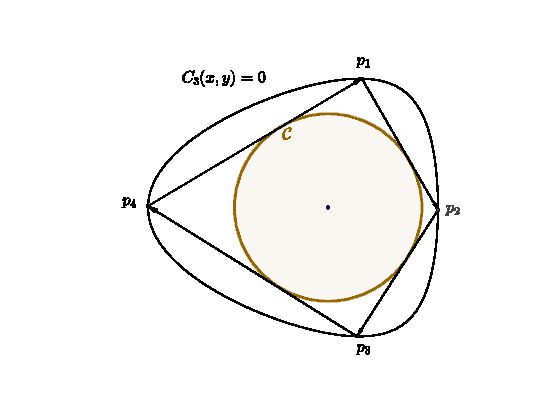
\includegraphics[scale=0.8]{chap_02/pics/chap2-040-darbouxC3C2.pdf}
\end{center}
\caption{Porism of 4-periodic orbits associated to $C_3(x,y)=0$ and the unit circle. }
\label{fig:C3C2}
\end{figure}

Consider a pair of conics (ellipses) defined by two quadratic forms $q_1(x,y,z)=\frac{x^2}{a_1^2}+\frac{y^2}{b_1^2}-z^2=0$ and $q_2(x,y,z)=\frac{x^2}{a_2^2}+\frac{y^2}{b_2^2}-z^2=0$ in projective coordinates $[x:y:z]$.

Let $f(t)=\sqrt{{\text det} (q_1+tq_2)}$ where

\begin{align*}
 q_i= \left(\begin{matrix}\frac{1}{a_i^2} &0 &0 \\
0 &\frac{1}{b_i^2} &0\\
0 & 0 &-1
\end{matrix}\right)
\end{align*}
